\documentclass[5p]{elsarticle}        % 5p gir 2 kolonner pr side. 1p gir 1 kolonne pr side.
\journal{fagl\ae rer}
\usepackage[T1]{fontenc} 				% Vise norske tegn.
\usepackage[norsk]{babel}				% Tilpasning til norsk.
\usepackage[utf8]{inputenc}             % selv puttet inn for ? kunne skrive norske tegn
\usepackage{graphicx}       				% For ? inkludere figurer.
\usepackage{amsmath,amssymb} 				% Ekstra matematikkfunksjoner.
\usepackage{siunitx}					% M? inkluderes for blant annet ? f? tilgang til kommandoen \SI (korrekte m?ltall med enheter)
	\sisetup{exponent-product = \cdot}      	% Prikk som multiplikasjonstegn (i steden for kryss).
 	\sisetup{output-decimal-marker  =  {,}} 	% Komma som desimalskilletegn (i steden for punktum).
 	\sisetup{separate-uncertainty = true}   	% Pluss-minus-form p? usikkerhet (i steden for parentes). 
\usepackage{booktabs}                     		% For ? f? tilgang til finere linjer (til bruk i tabeller og slikt).
\usepackage[font=small,labelfont=bf]{caption}		% For justering av figurtekst og tabelltekst.
\usepackage{comment}                            % for ? kunne kommentere i bolker (med \begin{comment} og \end{comment})
\usepackage[export]{adjustbox}            % for ? kunne plassere figurer bedre, h?yre venstre justering
\usepackage[below]{placeins}                      %tillatter bruk av \FloatBarrier ([above], [below])
\usepackage{pdfpages}

%\usepackage[section]{below}        %begrenser figuerer til sin section, kan bruker i stedet for \usepackage{placeins} 

% Denne setter navnet p? abstract til Sammendrag
\renewenvironment{abstract}{\global\setbox\absbox=\vbox\bgroup
\hsize=\textwidth\def\baselinestretch{1}%
\noindent\unskip\textbf{Sammendrag}
\par\medskip\noindent\unskip\ignorespaces}
{\egroup}


% Disse kommandoene kan gj?re det enklere for LaTeX ? plassere figurer og tabeller der du ?nsker.
\setcounter{totalnumber}{5}
\renewcommand{\textfraction}{0.05}
\renewcommand{\topfraction}{0.95}
\renewcommand{\bottomfraction}{0.95}
\renewcommand{\floatpagefraction}{0.35}

%%%%%%%%%%%%%%%%%%%%%%%%%%%%%%%%%%%%%%%%%%%%%%%%%%%%%%%%%%%%%%%%%%%%%%%%%
\begin{document}
\begin{frontmatter}
\title{Numerisk simulering av vekselvirkende partikler i sentralt gravitasjonsfelt.}
\author{H\aa kon Task{\'{e}}n}
\author{Paul Thrane}
%\address[fysikk]{Institutt for fysikk, Norges Teknisk-Naturvitenskapelige Universitet, N-7491 Trondheim, Norway.}
\begin{abstract}
Verlet integrasjon ble benyttet for \aa \ beregne partikkelbevegelser numerisk. Systemene som ble unders\o kt var henholdsvis en og to partikler i et sentralt gravitasjonsfelt, i topartikkel-systemet ble det tatt hensyn til gravitasjonskraft mellom partiklene.

\end{abstract}
\end{frontmatter}
%%%%%%%%%%%%%%%%%%%%%%%%%%%%%%%%%%%%%%%%%%%%%%%%%%%%%%%%%%%%%%%%%%%%%%%%%
\section{Teori og metode}
Bevegelsen til en partikkel i posisjon $\vec{r}_i$ med masse $m_i$, utsatt for en kraft $\vec{F}_i$, vil v\ae re bestemt av Newtons bevegelsesligning
\begin{equation}
m_i\frac{\mathrm{d}^2\vec{r}_i}{\mathrm{d}t^2}=\vec{F}_i.
\label{N2}
\end{equation}
Ligning \eqref{N2} kan skrives om til to koblede differensialligninger \cite{prosjektbeskrivelse}
\begin{equation}
\frac{\mathrm{d}\vec{v}_i}{\mathrm{d}t} = \vec{f}_i,
\label{n1}
\end{equation}
\begin{equation}
\frac{\mathrm{d}\vec{r}_i}{\mathrm{d}t}  = \vec{v}_i,
\label{n2}
\end{equation}
hvor $\vec{f}_i$ er kraft per masse p\aa \ partikkelen og $\vec{v}_i$ er hastigheten til partikkelen. Dersom initialbetingelser for $\vec{r}_i$ of $\vec{v}_i$ er kjent kan videre tidsforl\o p bestemmes ved numerisk l\o sning av \eqref{n1} og \eqref{n2} hvis $\vec{f}_i$ kan beregnes p\aa \ grunnlag av posisjon og hastighet til partikkelen. En metode som kan benyttes til dette er Verlet integrasjon, hvor $\vec{r}_i(t + \Delta t)$ og  $\vec{v}_i(t + \Delta t)$ beregnes etter kjennskap til $\vec{r}_i(t)$ ved f\o lgende ligninger\cite{prosjektbeskrivelse}
\begin{equation}
\vec{v}_i(t + \frac{\Delta t}{2}) = \vec{v}_i(t) + \vec{f}_i(t)\frac{\Delta t}{2},
\label{verlet1}
\end{equation}
\begin{equation}
\vec{r}_i(t + \Delta t) = \vec{r}_i(t) + \vec{v}_i(t + \frac{\Delta t}{2})\Delta t,
\end{equation}
\begin{equation}
\vec{v}_i(t + \Delta t) = \vec{v}_i(t + \frac{\Delta t}{2}) + \vec{f}_i(t + \Delta t)\frac{\Delta t}{2}.
\label{verlet2}
\end{equation}

Dersom potensialet til partikkelen, $V_i$, er kjent, kan kraften p\aa \ partikkelen beregnes ut fra sammenhengen $\vec{F}_i=-\nabla V_i$. I dette numeriske fors\o ket ble Verlet integrasjon benyttet for \aa \ beregne bevegelsene til \'{e}n og to massive partikler i bane rundt et sentralt legeme med masse $M$ og med gravitasjon som eneste vekselvirkende kraft. Det ble antatt at partiklenes masse, $m_1$ og $m_2$, var mye mindre enn $M$ slik at den sentrale massen st\aa r fast i origo. For \'{e}n enkelt partikkel blir potensialet
\begin{equation}
V_1 = \frac{GMm_1}{r_1},
\end{equation}
med $G$ en konstant som bestemmer styrken p\aa \ gravitasjonskraften. For to partikler blir potensialet p\aa \ partikkel $i$ ogs\aa \ p\aa virket av posisjonen til partikkel $j$
\begin{equation}
V_i = \frac{GMm_i}{r_i} + \frac{Gm_im_j}{|\vec{r}_i-\vec{r}_j|}.
\end{equation}

For \aa \ unders\o ke n\o yaktignheten av den numeriske metoden ble bevaring av energi og dreieimpuls unders\o kt. I tillegg ble de beregnede orbitalene til en enkelt partikkel sammenlignet med det eksakte uttrykket \cite{goldstein}
\begin{equation}
r = \frac{a(1-e^2)}{1+e\cos{(\theta - \theta')}},
\label{exact}
\end{equation}
hvor $(r,\theta)$ er posisjonen til partikkelen i polarkoordinater. Konstantene $a = -GM/2E$, og $e=(1+2El^2/m_1G^2M^2)^{0.5}$, der $E$ er energien til partikkelen og $l$ er dreieimpulsen om origo. Konstanten $\theta'$ spesifiseres av initialbetingelsene og kan settes lik null om en kun er interessert i hele orbitalen. Videre ble ogs\aa \ virialteoremet for \aa \ unders\o ke n\o yaktigheten av metoden da den gir en sammenheng mellom gjennomsnittlig kinetisk energi $\bar{T}$ og gjennomsnittlig potensiell energi $\bar{V}$ for en partikkel i et sentralt gravitasjonsfelt gitt ved\cite{goldstein}
\begin{equation}
\frac{\bar{T}}{\bar{V}}=-\frac{1}{2}.
\label{virial}
\end{equation}
Den numeriske metoden skal i utgangspunktet kunne benyttes p\aa \ alle initialbetingelser, men i dette tilfellet er det valgt \aa \ kun unders\o ke bundne tilstander, som har $E = T + V < 0$ \cite{goldstein}. Koden som er blitt benyttet for \aa \ l\o se ligning \eqref{n1} og \eqref{n2} er i appendiks.
%%%%%%%%%%%%%%%%%%%%%%%%%%%%%%%%%%%%%%%%%%%%%%%%%%%%%%%%%%%%%%%%%%%%%%%%%
\section{Resultat}
For kun en partikkel gir metoden en godt definert ellipseformet orbital, ettersom kun tilfeller med $E<0$ unders\o kes. Figur \ref{1pos} viser resultatet av en simulasjon sammen med tilh\o rende eksakte l\o sning, beregnet med ligning \eqref{exact}. Ved \aa \ teste for ulike initialbetingelser ble det funnet at et tidsteg p\aa \ under en promille av beregnet oml\o pstid som regel resulterte i en endring av total energi i st\o rrelsesorden $0.01\%$, mens et tidssteg p\aa \ omtrent $1\%$ av beregnet oml\o pstid resulterte i en endring av energi i st\o rrelsesorden $1\%$. Figur \ref{1energi} viser tilh\o rende total energi som funksjon av tid for systemet vist i figur \ref{1pos}. St\o rst endring i total energi ble funnet \aa \ skje n\aa r partikkelen befant seg n\ae rmest origo. For initialbetingelser som resulterte i god bevaring av total energi ble det ikke registrert noen endring av total dreieimpuls.

\begin{figure}[t] 
	\begin{center}
		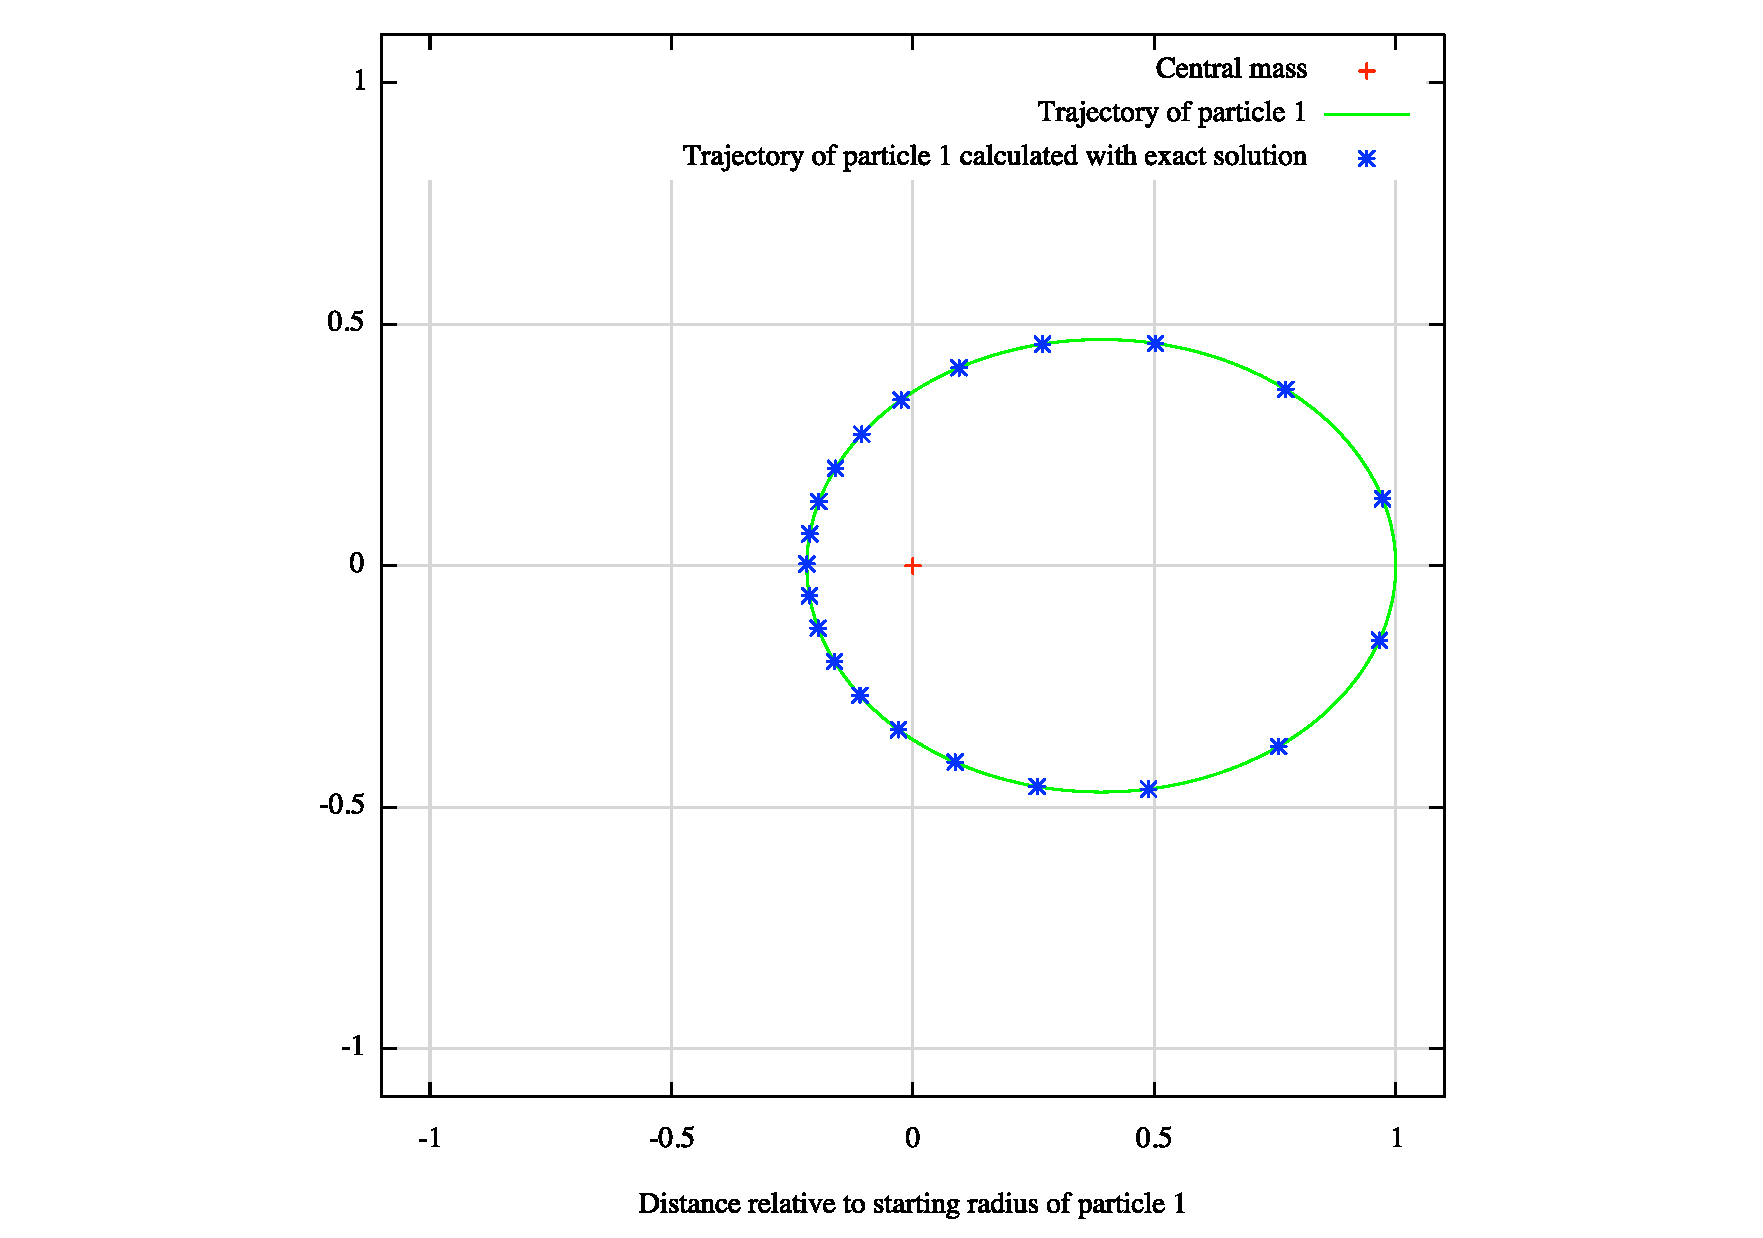
\includegraphics[width=.55\textwidth,center]{one_particle_position.pdf} 
	\end{center}
		\caption{Numerisk beregnet bevegelse for en partikkel i et sentralt gravitasjonsfelt vist med gr\o nn linje. Partikkelen beveger seg mot klokken med oml\o pstid 1,8. Eksakt bane for partikkelen er beregnet med ligning \eqref{exact} og er vist med bl\aa \ stjerner. Partikkelen starter i posisjon (1;0)} 
		\label{1pos} % Som med ligningen, er dette navnet vi refererer til.
\end{figure}
\begin{figure}[b] 
	\begin{center}
		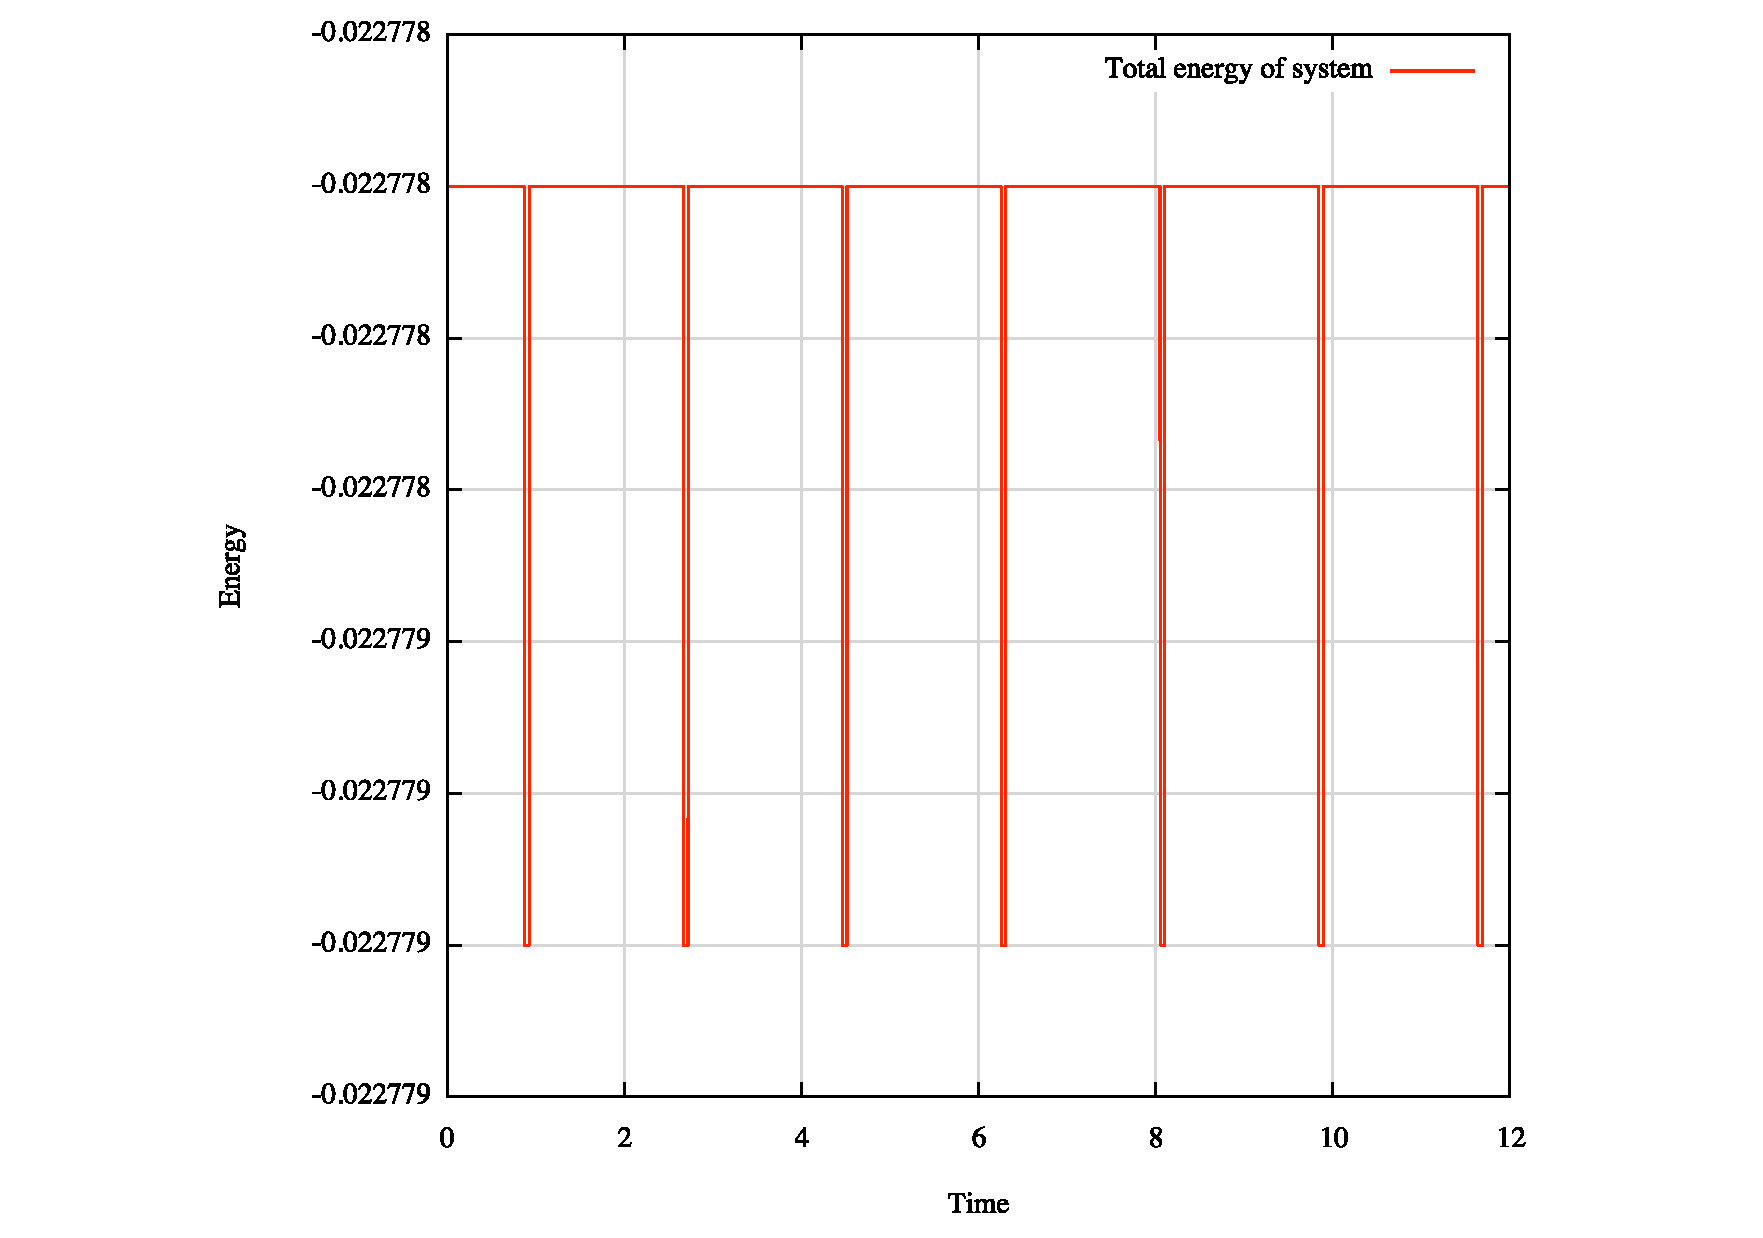
\includegraphics[width=.55\textwidth,center]{one_particle_energy.pdf} 
	\end{center}
		\caption{Total energi for en partikkel i et sentralt gravitasjonsfelt. Viser tidsforl\o p for system vist i figur \ref{1pos}.} 
		\label{1energi} % Som med ligningen, er dette navnet vi refererer til.
\end{figure}
$\bar{T}$ og $\bar{V}$ ble beregnet numerisk og sammenlignet med den teoretiske sammenhengen gitt av ligning \eqref{virial}. Generelt for initialbetingelser som resulterte i endring av total energi p\aa \ mindre enn $1\%$ ble det funnet at forholdet $\bar{T}/\bar{V}$ hadde et avvik fra teoretisk verdi p\aa \ mindre enn $0.1\%$.

For to vekselvirkende partikler i et sentralt gravitasjonsfelt ble n\o yaktigheten d\aa ligere. Dersom initialbetingelsene f\o rte partiklene i n\ae rheten av hverandre ble det ofte store avvik i total energi og ustabile orbitaler. Dersom initialbetingelsene ble bestemt slik at partiklene ikke kom for n\ae rme hverandre ble imidlertid banene ganske stabile, men med en regelmessig forskyvning av orbitalen il\o pet av simuleringen, figur \ref{2pos} viser et slikt tilfelle. Figur \ref{2energi} viser total energi som funksjon av tid for samme simulering, som p\aa \ det meste avviker $0.20\%$ fra startenergi. Endring av total dreieimpuls for samme simulering var for liten til \aa \ kunne leses av, noe som ogs\aa \ gjaldt andre simuleringer uten store avvik av total energi. Som for simulering av en partikkel ble det st\o rst endring av energi for de posisjonene der partiklene var i n\ae rheten av origo eller hverandre.

\begin{figure}[t] 
	\begin{center}
		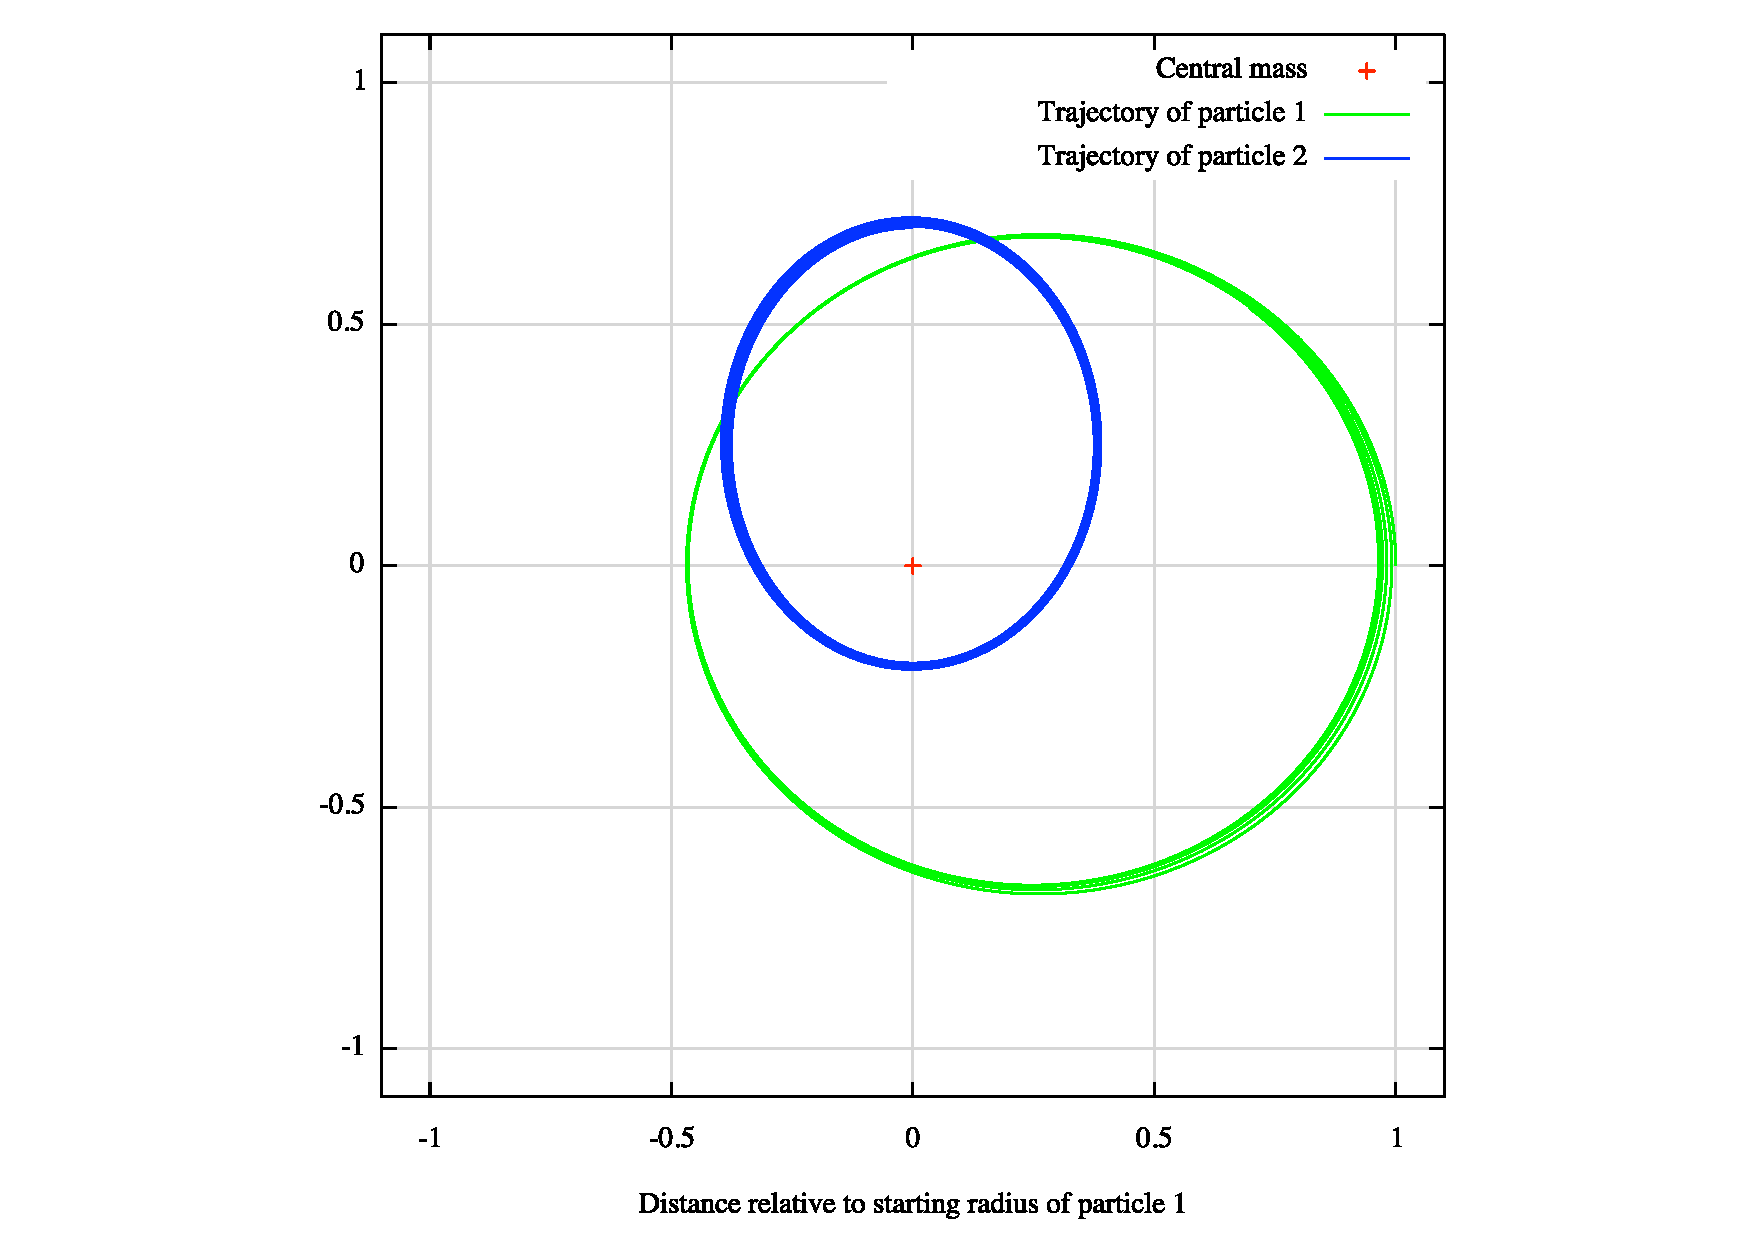
\includegraphics[width=.55\textwidth,center]{two_particles_position.pdf} 
	\end{center}
		\caption{Bevegelse for to vekselvirkende partikler i et sentralt gravitasjonsfelt. Partikkel 1 g\aa r mot klokken med oml\o pstid 3,0, partikkel 2 g\aa r mot klokken med oml\o pstid 1,4. Partikkel 1 starter i posisjon (1;0), og partikkel 2 starter i (0;0,7)} 
		\label{2pos} % Som med ligningen, er dette navnet vi refererer til.
\end{figure}
\begin{figure}[h] 
	\begin{center}
		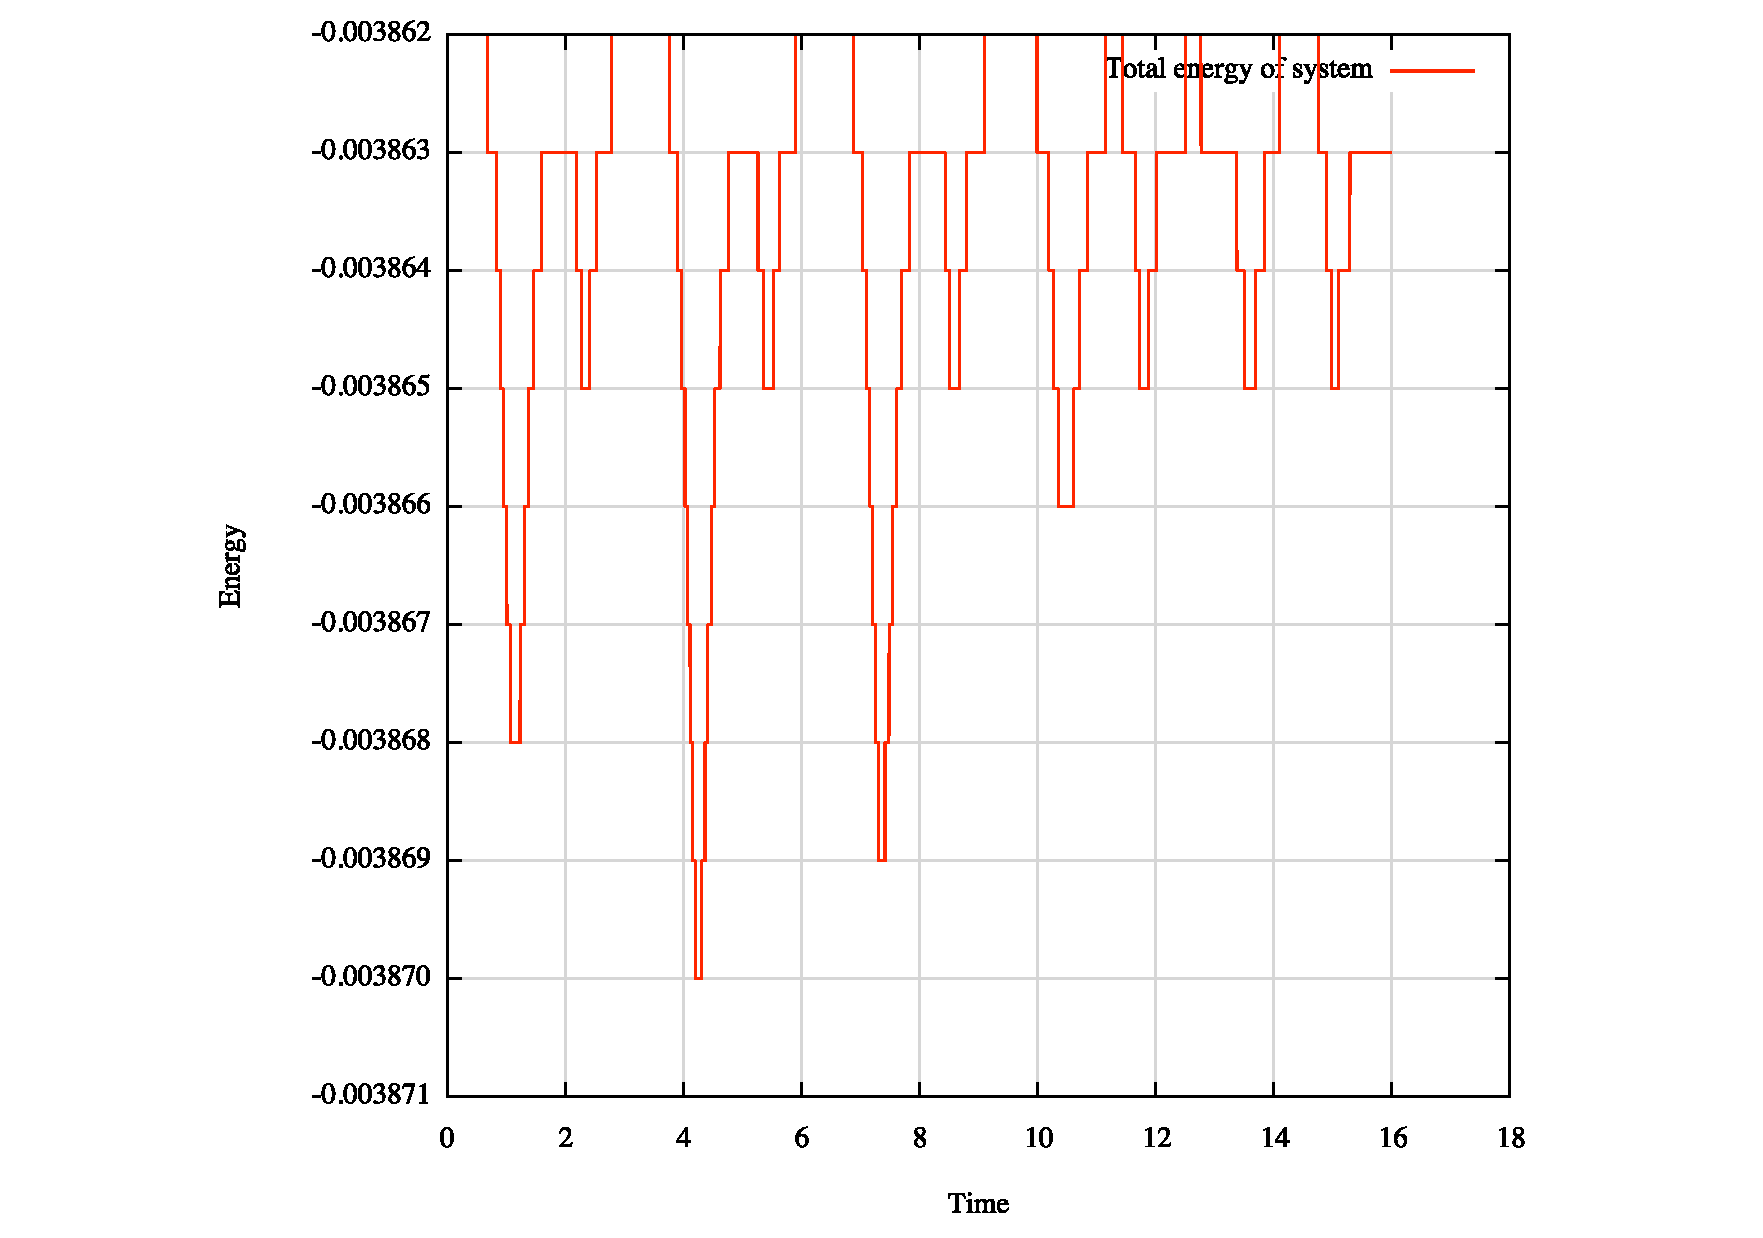
\includegraphics[width=.55\textwidth,center]{two_particles_energy.pdf} 
	\end{center}
		\caption{Total energi for system av to vekselvirkende partikler i et sentralt gravitasjonsfelt. Viser tidsforl\o p for system vist i figur \ref{2pos}} 
		\label{2energi} % Som med ligningen, er dette navnet vi refererer til.
\end{figure}

%%%%%%%%%%%%%%%%%%%%%%%%%%%%%%%%%%%%%%%%%%%%%%%%%%%%%%%%%%%%%%%%%%%%%%%%%
\section{Diskusjon og konklusjon}

For b\aa de simulering av en og to partikler er det tydelig at un\o yaktigheten i den numeriske metoden \o ker med kortere avstand mellom massene. Ved \aa \ unders\o ke figur \ref{1pos} og \ref{1energi} kan en se at endring av energi opptrer en gang per runde, og da i det punktet hvor partikkelen befinner seg n\ae rmest origo. Tilsvarende kan en se i figur \ref{2pos} og \ref{2energi} at energien til topartikkel-systemet endres mest i intervallet der orbitalene er i n\ae rheten av hverandre. Denne effekten kan forklares ved \aa \ se p\aa \ ligning \eqref{verlet1} og \eqref{verlet2}; feilen vil v\ae re avhengig av hvor raskt $\vec{f}_i$ endrer seg. Videre vil $\vec{f}_i$ endre seg raskest n\aa r partikkelen beveger seg fort og avstanden til andre masser er liten, som begge opptrer samtidig i n\ae rheten av andre masser.

Generelt virket metoden godt. For en enkelt partikkel samsvarte beregningene overens med ligning \eqref{exact} og ligning \eqref{virial}, samtidig som total energi og dreieimpuls var bevart uten \aa \ m\aa tte gj\o re $\Delta t$ veldig liten. For to vekselvirkende partikler ble metoden noe mer ustabil, men s\aa \ lenge initialbetingelser ble valgt slik at partiklene ikke beveget seg for n\ae rme hverandre ga beregningene svakt forkj\o vede orbitaler. For to partikler m\aa tte imidlertid $\Delta t$ i noen tilfeller gj\o res et par st\o rrelsesordner mindre for \aa \ oppn\aa \ samme bevaring av energi som for en enkelt partikkel.

%%%%%%%%%%%%%%%%%%%%%%%%%%%%%%%%%%%%%%%%%%%%%%%%%%%%%%%%%%%%%%%%%%%%%%%%%
\section*{Referanser}

\begin{thebibliography}{99}

\bibitem{prosjektbeskrivelse}
Prosjektbeskrivelse, Classical Mechanics TFY4345 - Computational Physics Project. NTNU, H\o sten 2015.

\bibitem{goldstein}
Goldstein, Safko, Poole. Classical Mechanics. Pearson Education Limited, Pearson new international edition, 3. utgave, 2014.

\end{thebibliography}

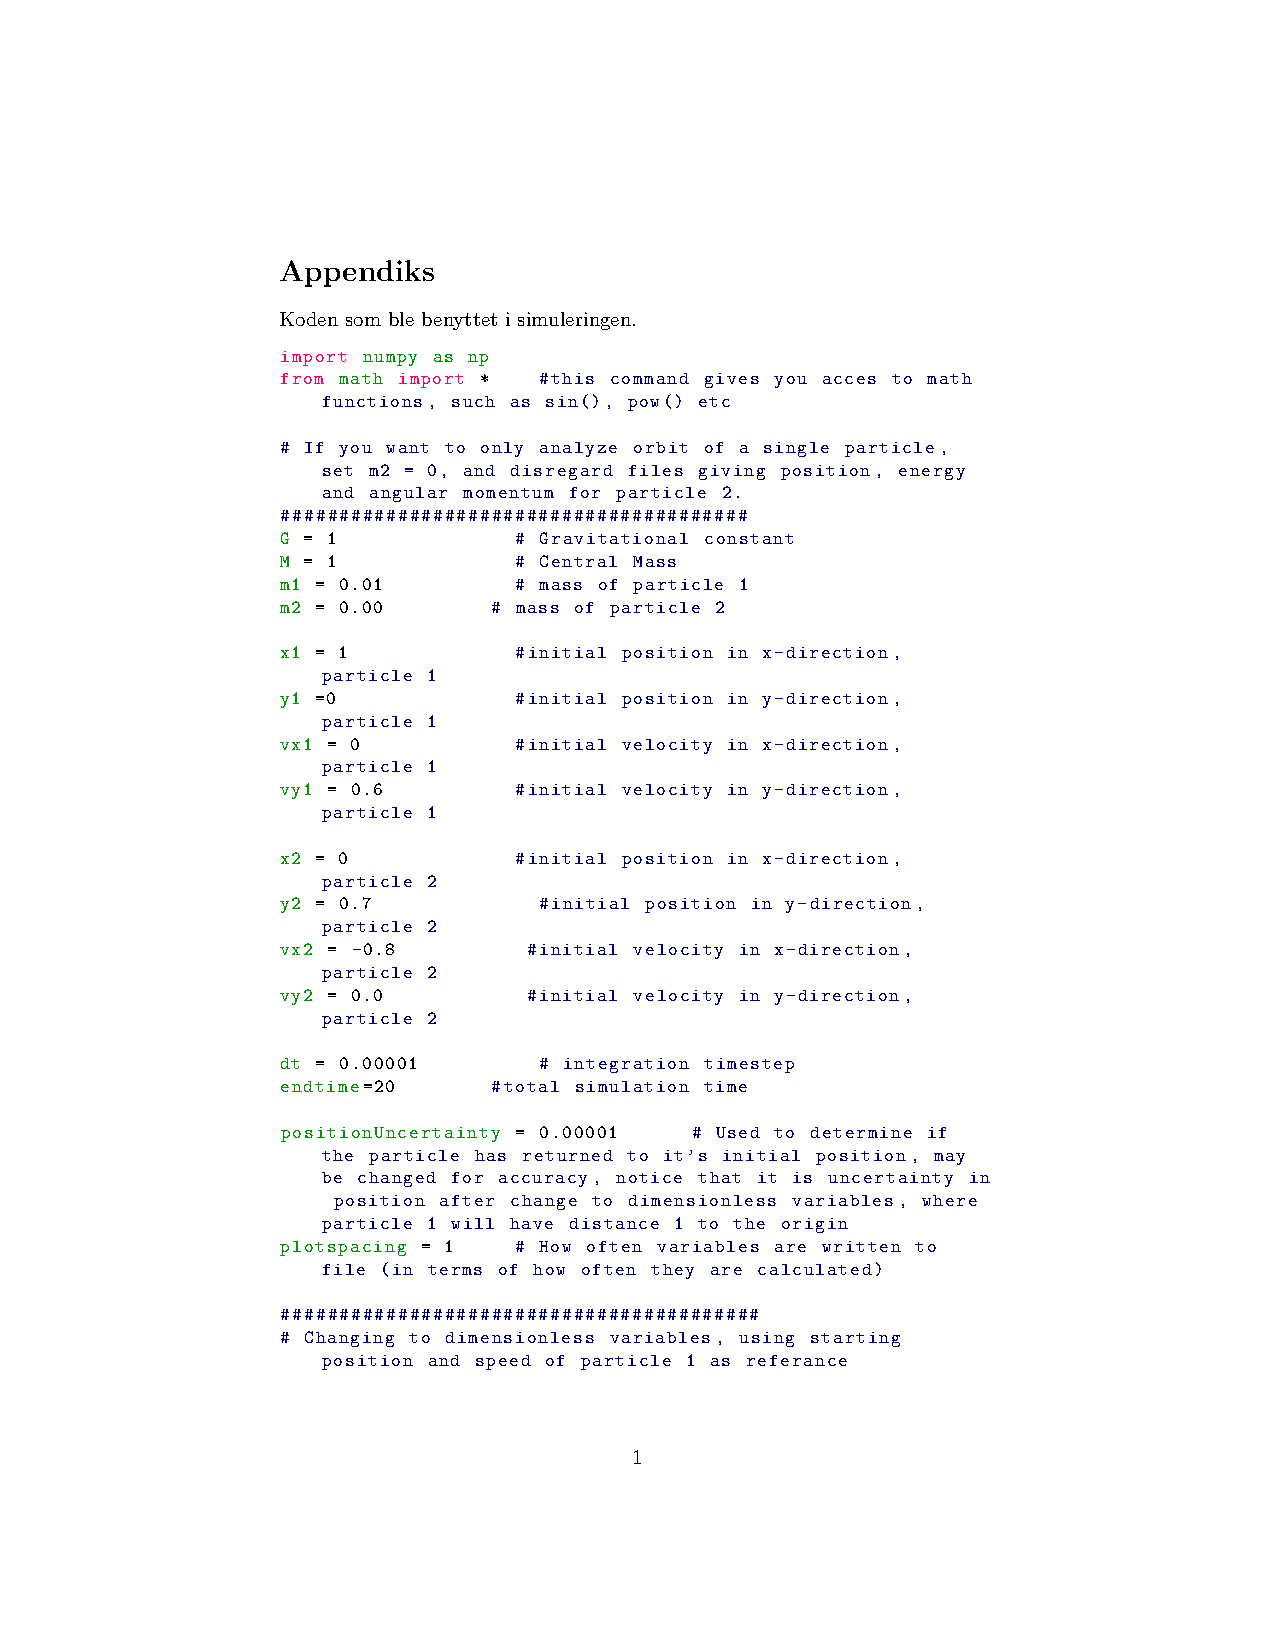
\includepdf[pages={1-},scale=1.2]{Appendix.pdf}


\end{document}